\chapter{Research Design and Methods} \label{ch:[chapter 5 label]}

\section{Overview}

In this research proposal, I have discussed the problem of search abandonment. I have noted that abandonment is partially due to search systems providing irrelevant results. This is because these systems have a weak understanding and employment of relevance. Guided by my research question, I propose a five-study research design to address this problem and improve our understanding of relevance in GIR. The relationships between studies are illustrated in figure \ref{fig:Methods_Overview}. Specifically, these studies will

\begin{enumerate}
    \item survey existing portals and record the state of faceted  search,
    \item analyze a portal for user search behavior, query topics, and latent concepts in queries that may suggest what users find relevant,
    \item analyze if and how latent concepts change with location (i.e., the location of a portal and/or datasets from a portal),
    \item modify an existing portal's search system to incorporate my findings on concept usage from the previous two studies, and
    \item evaluate the effectiveness of these modifications.
\end{enumerate}

\begin{figure}[H]
    \centering
    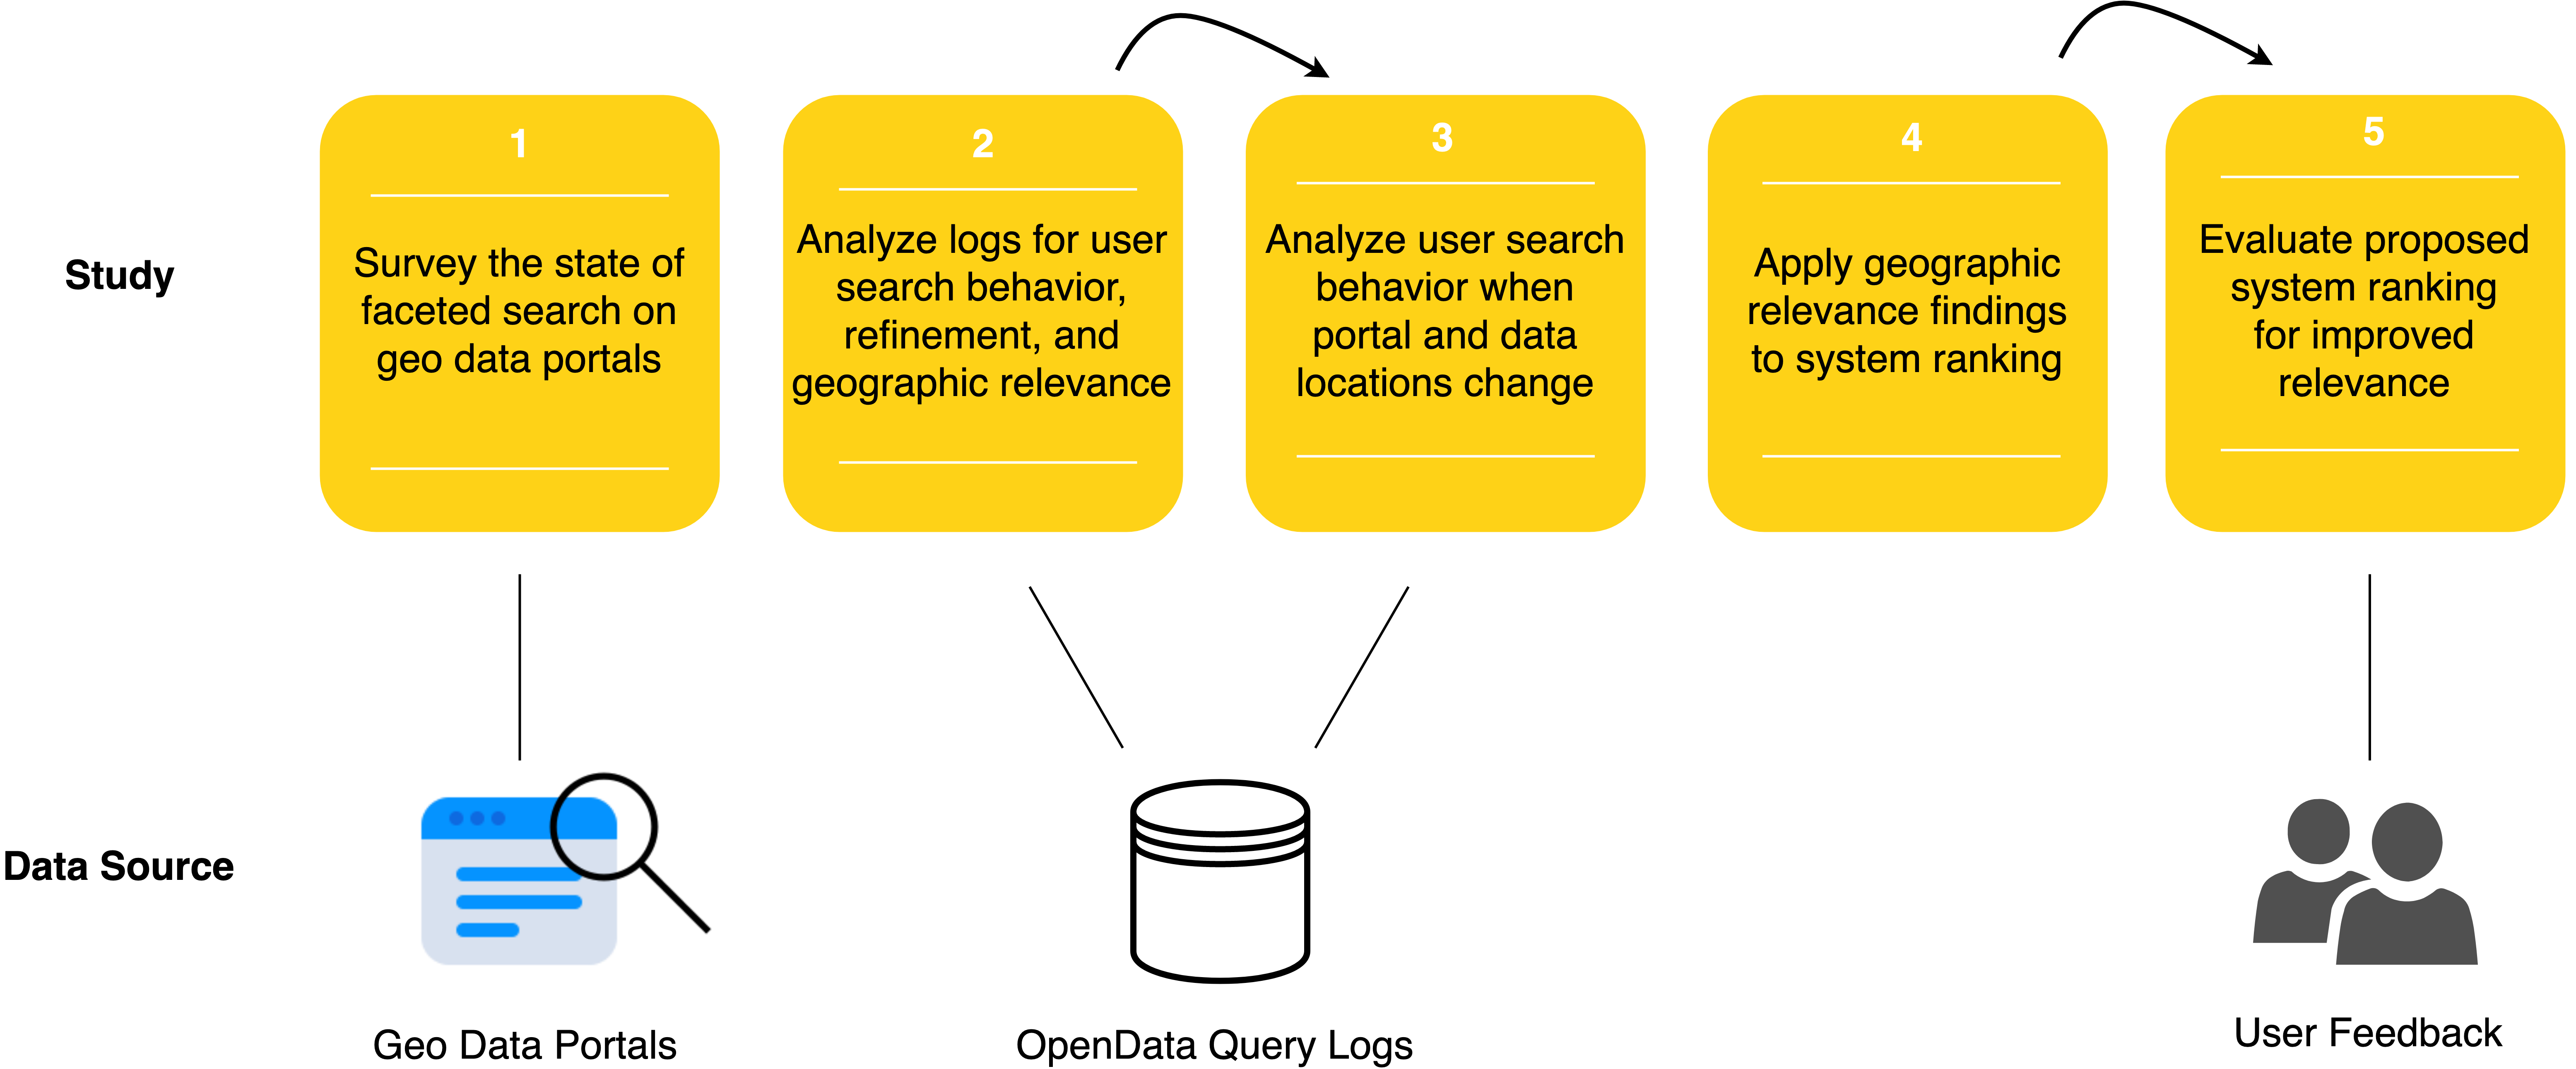
\includegraphics[width=1\textwidth]{../figures/Methods_Overview.png}
    \caption{Overview of research studies and their data sources. Studies progress by purpose including surveying the state of the art, interpreting search behavior, interpreting search behavior when location changes, applying knowledge about behavior, and evaluating the application. Arrows indicate a direct follow-up study.}
    \label{fig:Methods_Overview}
\end{figure}

\section{Surveying the State of Search in Geospatial Data Portals}

\subsection{Study Question}

The first step to reducing search abandonment to establish a baseline for search effectiveness. I am interested in understanding what facets users can control when they search and how search systems interpret and reason on user queries. By learning what portal users can do, I can identify gaps in their search systems. Therefore, my first research question is:
\linebreak

\emph{What is the state of faceted search and scoring/ranking functions on geospatial data portals?}

\subsection{Methods}

To answer this question, I will first survey the search facets of several commercial and academic portals including but not limited to Esri's OpenData, data.gov, census.gov, UCSB's Alexandria Digital Library, UCSB Library's new data portal, and Geoblacklight\footnote{\url{https://geoblacklight.org/}} enabled portals. I will record facets such as filtering by tags, drawing a region of interest on a map, or sorting alphabetically. Figure \ref{fig:Methods_OpenData} highlights the facets that a user controlled when searching and the ordered list of results.

Most search systems on portals do not publish their scoring/ranking functions, but many rely on open source data portals like CKAN\footnote{\url{https://ckan.org/}} and search tools like Apache Lucene\footnote{\url{https://lucene.apache.org/}}. They often leverage simple ranking models built on \gls{tf_idf} (\acrshort{TF_IDF}). TF–IDF ranks a document highly when it has a large number of similar words to a user's query, but those words aren't common in other documents. I expect that these search systems will apply similar functions possibly with minor customizations. For each portal, I will attempt several different information seeking tasks as if I were a typical user. I will simulate searching for data using specific queries for specific tasks. For example, in one scenario, I will simulate that I am a citizen who wants to reappraise their house and needs to find GIS data on parcels (to understand my property boundaries and coverage). After executing a query like "parcels", I will record the top 10 results and iteratively adjust the query to see if results change. Query adjustments will include: addition and removal of non-geographic, geographic, thematic and temporal terms, rearranging of terms, and the introduction and removal of terms indicative of the concepts that I hypothesized as being important. For example, I will add and remove spatial granularity keywords like "county" and "state", and density expressions such as "dense" or "even". Since data sparsity is likely to be an issue on some portals, I will trace several specific datasets on each portal and see how query adjustments affect their ranking.

\subsection{Expected Outcome}
The expected outcomes of this study will be threefold. First, this study will produce a list of observed options that affects search results on portals. This list will include all search facets and search weights, when knowable. A highly usable system strikes a balance between user control and system control. Systems with a large number of user controls dissuade serendipity, but few controls give little guidance. Second, this study will produce qualitative descriptions of how altering search terms affects results. Comparing queries and their responses will show if and how systems handle keywords differently. Third, this study will describe the observed deficiencies in existing systems including what queries and search facets yields irrelevant results, if any.

\begin{figure}[H]
    \centering
    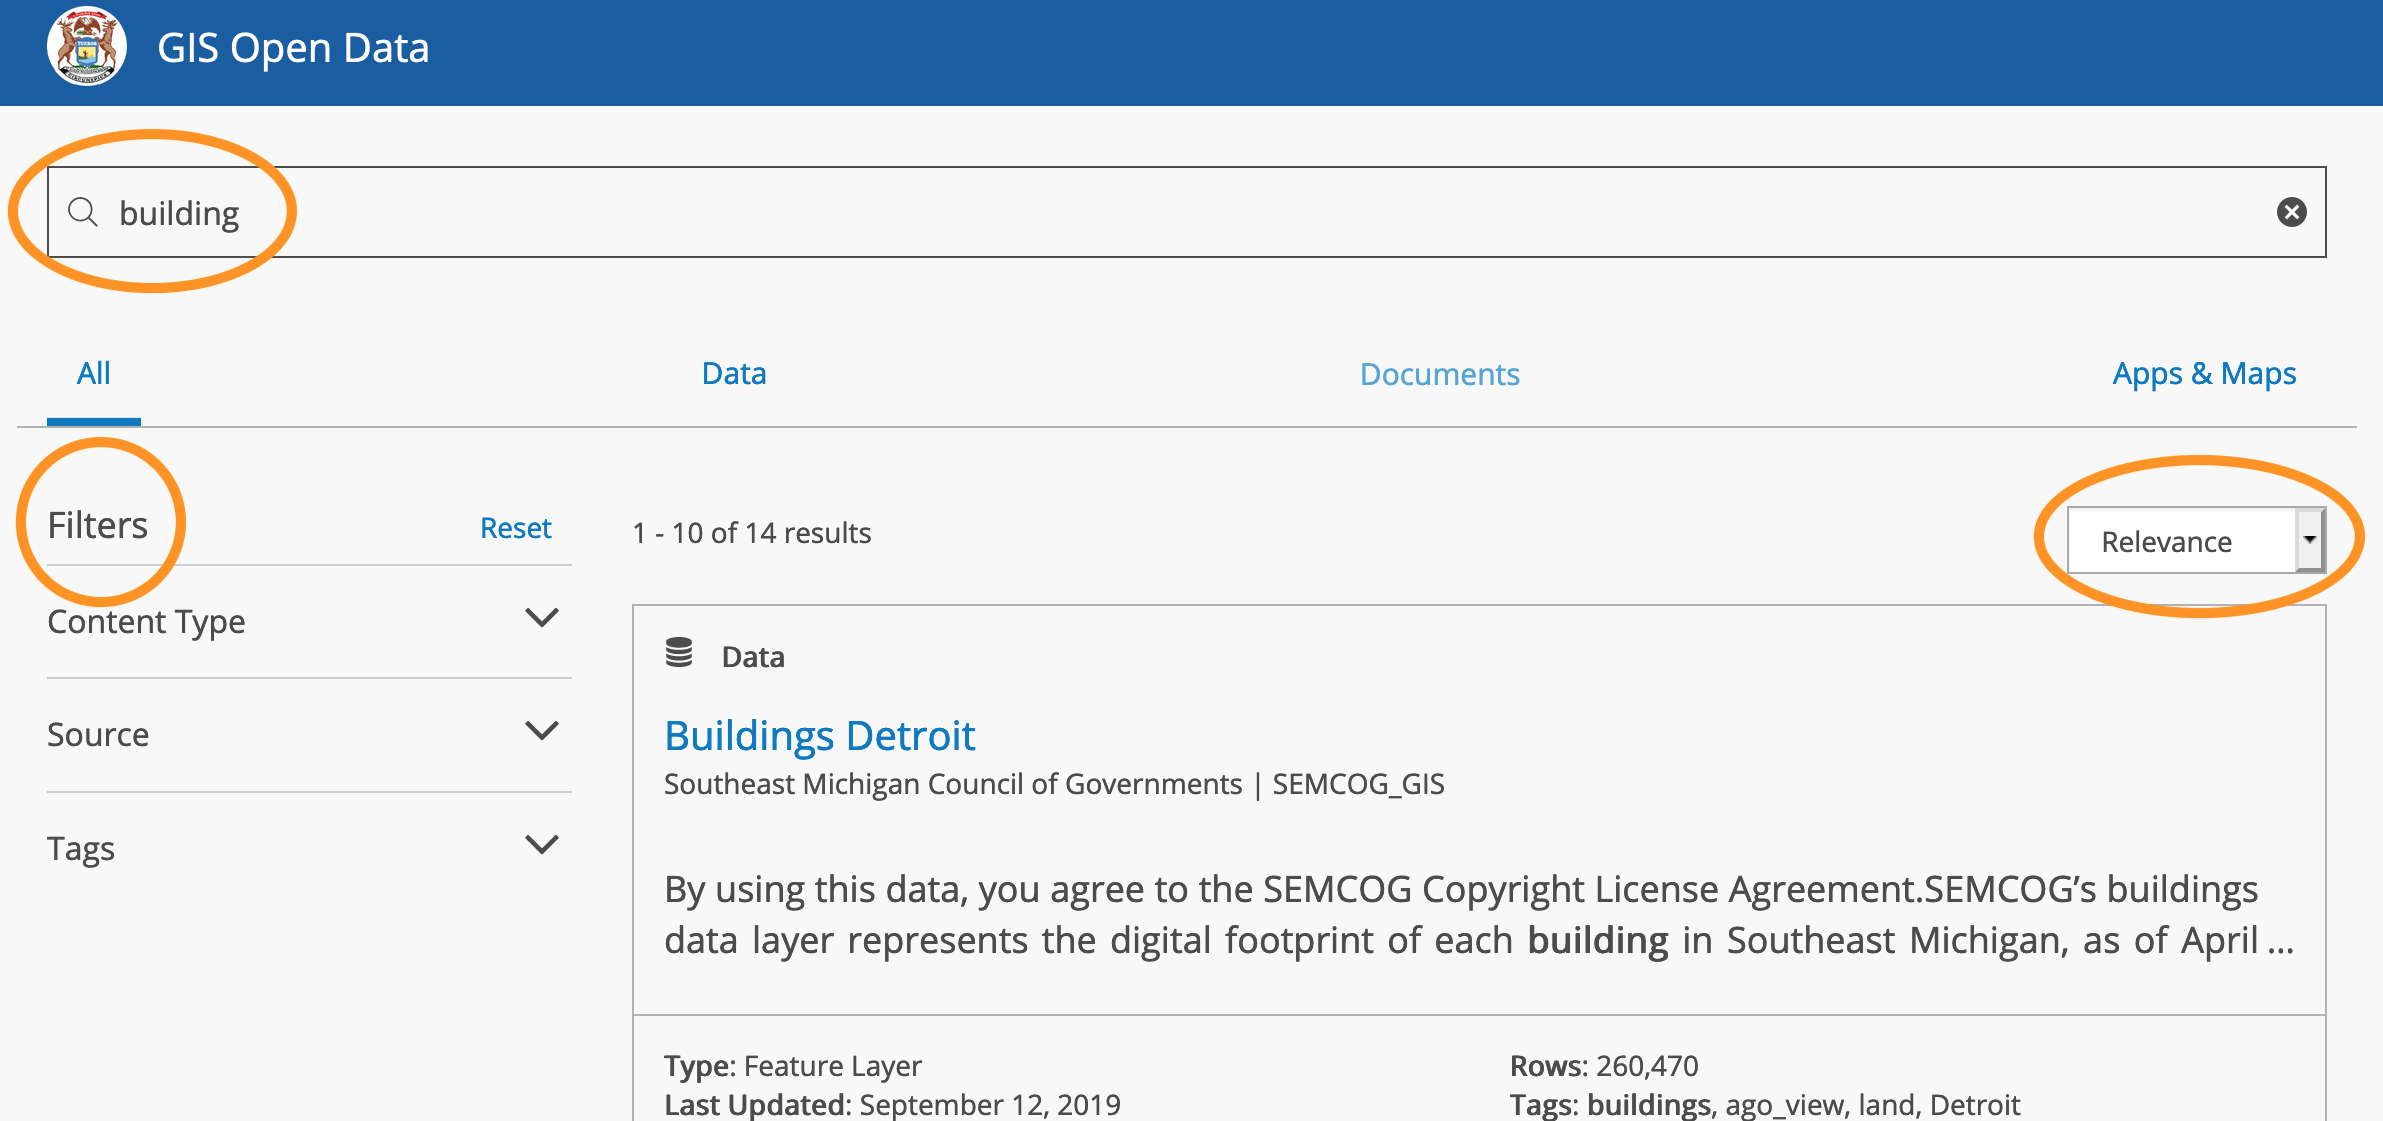
\includegraphics[width=1\textwidth]{../figures/Methods_OpenData.png}
    \caption{An example SERP from the Michigan OpenData portal. Orange highlights indicate facets that users control when searching. Surveying facets, surveying scoring/ranking functions, and observing SERP result changes from query changes are the research objectives of study 1. An ordered list of results are seen bottom right.}
    \label{fig:Methods_OpenData}
\end{figure}

\section{Search Behavior, Refinement and User's Query Concepts on Esri’s Geospatial OpenData Portals}

\subsection{Study Question}

Surveying the state of search shows us what users can do. But what do they actually do? The next logical step is to study user search behavior. The most common approach is to analyze query logs. Query logs record system interactions. These interactions including query executions, search refinements, page clicks, navigation, downloads, dwell time, and search exits are proxies for search behavior. Ultimately, they suggest what users commonly do, what they’re asking for, where they get stuck, and what they did before they abandoned their search. Although relevance cannot be directly quantified from query logs, certain behaviors are commonly used as relevance proxies. Query phrases are particularly important. They are an articulation of an information need. Analyzing word and phrase usage is very important to understanding the topics and concepts that are relevant to user needs. In this study, in addition to describing general search behavior and refinement, I want to answer the question:
\linebreak

\emph{Which concepts do people use implicitly and explicitly when searching for geospatial data, and how do they relate to search behavior and search refinement?}

\subsection{Data}

In this study, I will use several related datasets. I will primarily analyze text query logs from popular portals–Esri’s OpenData sites. This dataset is provided by Esri’s DC R+D office who develops OpenData. It includes over 1.5 million unique query strings, over 1 million unique search refinements, and dozens of ancillary attributes for each query string including page depth (i.e., the number of SERP results clicked), search dwell time, percentage of search abandonment, and percentage of goal conversions (i.e., percentage of downloads) among others. I have pre-processed these data and indexed them a PostgreSQL\footnote{\url{https://www.postgresql.org/}} database for use in full-text analysis. Unfortunately, due to privacy restrictions on the Google Analytics\footnote{\url{https://analytics.google.com/analytics/web/}} platform where these data originated, I am unable to extract individual search sessions at scale which would include what a specific user searches, clicks, and downloads. Therefore, the dataset is comprised of aggregates and averages. However, in the near future, I should have access to a second dataset called ELB logs. These logs are session-like data that records user navigation, such as what result a user clicks on following a query. They will require coalescing to resemble search sessions. These data are critical because clicks will be the foundation for constructing relevance judgements (see studies 4 and 5). The last dataset contains geospatial documents, which are publicly available via on OpenData’s \gls{application_programming_interface} (\acrshort{API}). All datasets will be filtered to contain only English queries and documents that are to US-based OpenData sites as a way of controlling cultural and linguistic variation in behavior. These datasets combined will include the three components necessary for IR evaluation–queries, documents, and relevance judgements.

\subsection{Methods}

Analyzing query logs can take dozens of different natural language processing data mining approaches. I will follow several classical IR and GIR approaches. As discussed previously, once queries are properly parsed and annotated, classical analysis starts simple by analyzing the frequency, distribution, and covariance of query terms and query phrases. Then, domain-specific analysis attempts to identify patterns across queries, such as the frequency of specific geographic named entities, parts of speech distributions, and more. Typically syntactic analysis then gives way to semantic analysis. This includes identifying topics, sentiment, and identifying explicit and implicit concepts embedded in search queries. This is conducted using robust tools for topic modeling, latent semantic analysis, and word/document embedding into vector space. Lastly, behavioral inferences are made based on the relation between findings from syntactic and semantic analysis and how a user progresses through the search process. For example, a researcher may want to know which query terms and topics most often lead to high search abandonment and/or short dwell time.

I am particularly interested in what explicit and implicit concepts users use in their queries. Therefore, I will attempt to enumerate these concepts and see how they relate to search behavior by observing two parts of my first dataset–text queries and behavior proxies (e.g, search dwell time). First, I will analyze query phrase and term usage across the entire corpus using NLP text processing techniques developed in \cite{Sanderson2007} \cite{Dittrich2015} \cite{Derungs2016} \cite{Gablasova2017} \cite{Hamzei2019b}. I will record typical IR descriptive statistics including: frequency and length of phrases, n-grams, and terms, frequency of parts of speech, and phrase dependencies. I will also attempt to model themes using the popular \gls{Latent_Dirichlet_Allocation} (\acrshort{LDA}) model and a short-text model called \gls{Dirichlet_Multinomial_Mixture} (\acrshort{GSDMM}). I will also describe general search behavior such as search trends (i.e., how OpenData usage has changed over time).

Second, I will look for the same patterns within and between queries. To start, I will normalize and label query terms using the same NLP methods used on the corpus and look for interactions between spatial, temporal, and thematic terms. To do this, queries are typically converted into a \gls{bag_of_words} (\acrshort{BoW}) model where word order doesn't matter but term frequency does. Then, using the \gls{vector_space_model}, feature vectors are created for the query where each feature is a BoW unigram (query term). The vector space model allows for easy similarity comparison between words and queries by calculating the cosine similarity of features. Using the vector space model, I will look for similarities between query vectors and attempt to cluster queries thematically. Since search themes widely vary, I will use a second method for comparing thematic similarity between queries. I will use ConceptNet\footnote{\url{http://conceptnet.io/}}, a semantic network built on vocabularies like Wordnet\footnote{\url{https://wordnet.princeton.edu/}}, to expand queries and reinforce findings from the vector space model. There is debate about directly applying semantic networks, but I will assume that network distance and hierarchy levels are indicative of semantic distance (within a certain threshold). I have also considered applying a geo-ontology to classify query terms, but this is not certain. Once themes are modeled, I will attempt to see how they covary with geographic and spatial terms. To do this, I will geoparse and geocode queries to label place names, addresses, and spatial qualifiers (i.e., directions like “north”, relations like “inside”, topology like “next to”, etc.) based on pre-existing (e.g., Geonames) and custom-built databases and tools (e.g., OpenAddresses). Then, I will record if and how spatial and thematic terms covary.

Third, since query refinement is common and indicative that SERP results aren't relevant, I will analyze refinement patterns. Specifically I will look for query expansions, contractions, and reformulations. I will record if and how users spatially refine such as adding a zip code to an address (i.e., geocorrection) or changing place names (i.e., georeformulation), and how users thematically refine, once again using ConceptNet and a threshold to set theme limits.

Fourth, based on findings from the previous three steps, I will see how query terms relate to search behavior, page progression, and abandonment. For each unique query in the corpus, there is a record for search depth, percent search exit (i.e., the rate that users leave a site after searching), search duration (i.e., the amount of time that a user spends examining results after a search), goal conversions (i.e., the rate of a goal being completed, such as downloading a dataset or making a call to the OpenData API). 

Throughout these steps, I will record the types and frequencies of explicit and implicit concepts embedded in user queries. After manually annotating these concepts for a subset of the data, I will look to see if and how they change based on the variations previously discussed (e.g., by query length, with specific query terms, after query refinement, etc.). I acknowledge that concepts can be anything and everything. I am specifically interested thematic (explicit) and latent (implicit) that could be deduced by a human reading query text. For example, the query "2008 population density by congressional district" has several explicit and implicit concepts. The explicit concepts are a timeframe (i.e., "2008"), and specific spatial unit type (i.e., the administrative unit "congressional district"). Implicit concepts give context to the themes in a query. The implicit concepts are temporal granularity (i.e., a specific year), spatial granularity (i.e., an administrative unit), and spatial configuration (i.e., density). These concepts are not pre-determined and will be expectantly debated. I believe that implicit concepts frequently found in queries that proceed search abandonment are likely neglected by the system. They should be recognized as valuable and will be incorporated into relevance ranking (see study 4).

\subsection{Expected Outcome}
The expected outcome of this study will be fourfold including 
\begin{enumerate}
    \item a qualitative and quantitative description of general search patterns on Esri OpenData portals,
    \item a quantitative description of query and term frequency, query themes and geographic and spatial term usage,
    \item a quantitative description of the types and frequencies of query refinements and geo-refinements and how they relate to general search behaivor,
    \item and a qualitative description and list of the concepts searchers use that may be indicative of what they consider relevant to their search.
\end{enumerate}

The majority of my current research is invested in this study. I have considered that this study may require being broken down into several smaller studies.

\section{Impacts of Location on Search Behavior in Search of Geographic  Datasets}
\subsection{Study Question}
\subsection{Data}
\subsection{Methods}
\subsection{Expected Outcome}

\section{An Experimental Study on the Effectiveness of Introducing Relevance Criteria in Geographic Information Retrieval}
\subsection{Study Question}
\subsection{Data}
\subsection{Methods}
\subsection{Expected Outcome}

\section{Evaluating the Effectiveness of a Geographically-Oriented Search Rank Algorithm}
\subsection{Study Question}
\subsection{Data}
\subsection{Methods}



Goal conversions will be used as a proxy for relevance judgements. Note that I make an important assumption. Since I do not have relevance judgements (the typical third component of query–document–relevance judgement in a test collection) nor will I manually annotate relevance judgements, I will use proxies as relevance judgements.

A download will mean that the document downloaded is relevant and that the search session is successful. Alternatively, search exits will mean that the datasets are not relevant. For example, if a query is issued with no refinements and results in a downloaded dataset, this can be considered a successful search session. If a user refines their search multiple times and doesn’t download a dataset, this is an example of an unsuccessful session. I will separate and compare the results between successful and unsuccessful sessions. As mentioned previously, this method will be used for creating relevance judgements until I have access to the ELB logs.

Results will be more meaningful once I curate the ELB logs because it more closely resembles search sessions where a user executes a query, clicks on certain results, and ultimately downloads a dataset or abandons the session. In this case, clicks will be used in conjunction with goal conversions to create relevance judgements. Clicks are highly variable and literature suggests that a click does not mean that a result is relevant. However, a click, particularly if it isn’t to the top result, indicates preference and that the result is relatively more valuable than the top result. Therefore, clicks can be used in a probabilistic model for calculating relevance scores. Furthermore, clicks can be combined with more concrete relevance proxies, such as goal conversions discussed earlier. It is likely that this method for determining relevance judgements will be improved before this study is complete. Ultimately, the ELB logs will be used to create a test collection of query¬–document–relevance judgement triples. In theory, this test collection, were it to be made public, would be useful for future GIR evaluations.


Figure \ref{fig:Methods_Evaluation}

\subsection{Expected Outcome}

\begin{figure}[H]
    \centering
    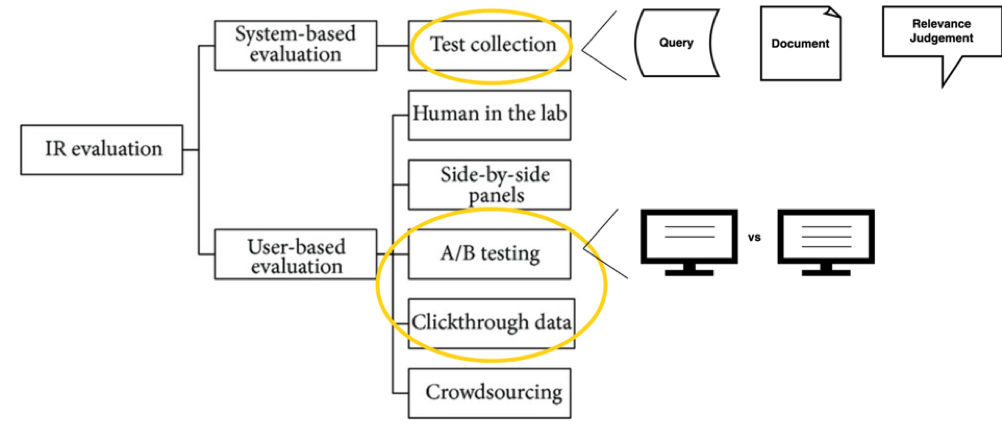
\includegraphics[width=1\textwidth]{../figures/Methods_Evaluation.png}
    \caption{Classification of IR evaluation approaches adapted from \cite{Samimi2014}. Yellow highlights indicate the evaluation approaches used in this study. A test collection comprises a query, document, and relevance judgement for each query-document pair. A/B testing assigns users to either an A (control) or B (modified) search system and compares their behavior. I will also add an option for self-reported relevance on each SERP result. Click-through data, parsed from query logs in study 2, will be used to cross-reference A/B testing results.}
    \label{fig:Methods_Evaluation}
\end{figure}